% Options for packages loaded elsewhere
\PassOptionsToPackage{unicode}{hyperref}
\PassOptionsToPackage{hyphens}{url}
\PassOptionsToPackage{dvipsnames,svgnames,x11names}{xcolor}
%
\documentclass[
  Crown,
  times,
  sageh]{sagej}
\usepackage{amsmath,amssymb}
\usepackage{iftex}
\ifPDFTeX
  \usepackage[T1]{fontenc}
  \usepackage[utf8]{inputenc}
  \usepackage{textcomp} % provide euro and other symbols
\else % if luatex or xetex
  \usepackage{unicode-math} % this also loads fontspec
  \defaultfontfeatures{Scale=MatchLowercase}
  \defaultfontfeatures[\rmfamily]{Ligatures=TeX,Scale=1}
\fi

\ifPDFTeX\else
  % xetex/luatex font selection
  \fi
\usepackage[T1]{fontenc}
\usepackage{helvet}
\renewcommand\familydefault{\sfdefault}


% Use upquote if available, for straight quotes in verbatim environments
\IfFileExists{upquote.sty}{\usepackage{upquote}}{}
\IfFileExists{microtype.sty}{% use microtype if available
  \usepackage[]{microtype}
  \UseMicrotypeSet[protrusion]{basicmath} % disable protrusion for tt fonts
}{}
\makeatletter
\@ifundefined{KOMAClassName}{% if non-KOMA class
  \IfFileExists{parskip.sty}{%
    \usepackage{parskip}
  }{% else
    \setlength{\parindent}{0pt}
    \setlength{\parskip}{6pt plus 2pt minus 1pt}}
}{% if KOMA class
  \KOMAoptions{parskip=half}}
\makeatother
\usepackage{xcolor}
\usepackage{longtable,booktabs,array}
\usepackage{calc} % for calculating minipage widths
% Correct order of tables after \paragraph or \subparagraph
\usepackage{etoolbox}
\makeatletter
\patchcmd\longtable{\par}{\if@noskipsec\mbox{}\fi\par}{}{}
\makeatother
% Allow footnotes in longtable head/foot
\IfFileExists{footnotehyper.sty}{\usepackage{footnotehyper}}{\usepackage{footnote}}
\makesavenoteenv{longtable}
\usepackage{graphicx}
\makeatletter
\def\maxwidth{\ifdim\Gin@nat@width>\linewidth\linewidth\else\Gin@nat@width\fi}
\def\maxheight{\ifdim\Gin@nat@height>\textheight\textheight\else\Gin@nat@height\fi}
\makeatother
% Scale images if necessary, so that they will not overflow the page
% margins by default, and it is still possible to overwrite the defaults
% using explicit options in \includegraphics[width, height, ...]{}
\setkeys{Gin}{width=\maxwidth,height=\maxheight,keepaspectratio}
% Set default figure placement to htbp
\makeatletter
\def\fps@figure{htbp}
\makeatother
\setlength{\emergencystretch}{3em} % prevent overfull lines
\providecommand{\tightlist}{%
  \setlength{\itemsep}{0pt}\setlength{\parskip}{0pt}}
\setcounter{secnumdepth}{5}
% Make \paragraph and \subparagraph free-standing
\ifx\paragraph\undefined\else
  \let\oldparagraph\paragraph
  \renewcommand{\paragraph}[1]{\oldparagraph{#1}\mbox{}}
\fi
\ifx\subparagraph\undefined\else
  \let\oldsubparagraph\subparagraph
  \renewcommand{\subparagraph}[1]{\oldsubparagraph{#1}\mbox{}}
\fi
\usepackage[perpage]{footmisc}
\makeatletter
\@ifpackageloaded{caption}{}{\usepackage{caption}}
\AtBeginDocument{%
\ifdefined\contentsname
  \renewcommand*\contentsname{Table of contents}
\else
  \newcommand\contentsname{Table of contents}
\fi
\ifdefined\listfigurename
  \renewcommand*\listfigurename{List of Figures}
\else
  \newcommand\listfigurename{List of Figures}
\fi
\ifdefined\listtablename
  \renewcommand*\listtablename{List of Tables}
\else
  \newcommand\listtablename{List of Tables}
\fi
\ifdefined\figurename
  \renewcommand*\figurename{Figure}
\else
  \newcommand\figurename{Figure}
\fi
\ifdefined\tablename
  \renewcommand*\tablename{Table}
\else
  \newcommand\tablename{Table}
\fi
}
\@ifpackageloaded{float}{}{\usepackage{float}}
\floatstyle{ruled}
\@ifundefined{c@chapter}{\newfloat{codelisting}{h}{lop}}{\newfloat{codelisting}{h}{lop}[chapter]}
\floatname{codelisting}{Listing}
\newcommand*\listoflistings{\listof{codelisting}{List of Listings}}
\makeatother
\makeatletter
\makeatother
\makeatletter
\@ifpackageloaded{caption}{}{\usepackage{caption}}
\@ifpackageloaded{subcaption}{}{\usepackage{subcaption}}
\makeatother
\ifLuaTeX
  \usepackage{selnolig}  % disable illegal ligatures
\fi
\usepackage[]{natbib}
\bibliographystyle{SageH}
\IfFileExists{bookmark.sty}{\usepackage{bookmark}}{\usepackage{hyperref}}
\IfFileExists{xurl.sty}{\usepackage{xurl}}{} % add URL line breaks if available
\urlstyle{same}
\hypersetup{
  pdftitle={Land and Language in Australian Romanticism},
  pdfauthor={Michael Falk},
  pdfkeywords={Harpur, Charles; Dunlop, Eliza Hamilton; Wulatji;
Romanticism; philosophy of language; terra nullius},
  colorlinks=true,
  linkcolor={blue},
  filecolor={Maroon},
  citecolor={Blue},
  urlcolor={Blue},
  pdfcreator={LaTeX via pandoc}}

\usepackage{float}
\makeatletter
\let\oldlt\longtable
\let\endoldlt\endlongtable
\def\longtable{\@ifnextchar[\longtable@i \longtable@ii}
\def\longtable@i[#1]{\begin{figure}[H]
\onecolumn
\begin{minipage}{\columnwidth}
\oldlt[#1]
}
\def\longtable@ii{\begin{figure}[H]
\onecolumn
\begin{minipage}{\columnwidth}
\oldlt
}
\def\endlongtable{\endoldlt
\end{minipage}
% \twocolumn
\end{figure}}
\makeatother

\title{Land and Language in Australian Romanticism}
\author{Michael Falk\affilnum{1}}

\affiliation{
    \affilnum{1} University of Melbourne \\
  }

\corrauth{}

\email{}

\begin{abstract}
Eliza Hamilton Dunlop (1796-1880) and Charles Harpur (1813-1867) were
two of the most important Romantic poets of colonial New South Wales. In
this article, I consider their engagement with Indigenous Australian
languages. In `Native Song' (1848), Dunlop provides a transcription and
translation of verse composed by her informant Wulatji (fl.~1840s), a
famous Awabakal poet. In \emph{The Kangaroo Hunt} (c.~1844), Harpur
enriches his description of Australian landscapes with a dozen words
learned from Darkinyung, Gamilaraay and Wonnarua informants. I contrast
Dunlop's universalist approach to Indigenous langauge with Harpur's
particularist approach, and contextualise their poetry in British
philosophy of language. Dunlop and Harpur use Indigenous language to
present Australia as a land steeped in poetry, but their recognition of
Indigenous poetry undermines their own attempts to make themselves at
home in the colony.
\end{abstract}
\keywords{Harpur, Charles; Dunlop, Eliza Hamilton; Wulatji; Romanticism;
philosophy of language; terra nullius, Harpur, Charles; Dunlop, Eliza
Hamilton; Wulatji; Romanticism; philosophy of language; terra nullius}



\begin{document}


\maketitle


\maketitle
\begin{abstract}
Eliza Hamilton Dunlop (1796-1880) and Charles Harpur (1813-1867) were
two of the most important Romantic poets of colonial New South Wales. In
this article, I consider their engagement with Indigenous Australian
languages. In `Native Song' (1848), Dunlop provides a transcription and
translation of verse composed by her informant Wulatji (fl.~1840s), a
famous Awabakal poet. In \emph{The Kangaroo Hunt} (c.~1844), Harpur
enriches his description of Australian landscapes with a dozen words
learned from Darkinyung, Gamilaraay and Wonnarua informants. I contrast
Dunlop's universalist approach to Indigenous langauge with Harpur's
particularist approach, and contextualise their poetry in British
philosophy of language. Dunlop and Harpur use Indigenous language to
present Australia as a land steeped in poetry, but their recognition of
Indigenous poetry undermines their own attempts to make themselves at
home in the colony.
\end{abstract}

\renewcommand*\contentsname{Table of contents}
{
\hypersetup{linkcolor=}
\setcounter{tocdepth}{3}
\tableofcontents
}
\subsection{Introduction}\label{introduction}

To occupy Australia, its European invaders had to name it. This was not
merely a matter of naming places, though that of course was crucial.
They also needed to name the things the made the places. They needed to
name the trees that dropped their autumn bark, the deer-like creatures
that hopped on two legs, the fires that ripped through crackling
scrubland. They needed to name the fickle weather, the whirling dust,
the intermittent streams. They needed to name hundreds of parrots and
pigeons and snakes and dragons. They needed to name the people from whom
they took the land. To conquer Australia, they ``conquered space.'' With
a touch of the namer's wand, they changed a strange land ``into a
familiar world of routes and places'' \citep[83]{tuan_space_1977}.

The invaders mined Indigenous languages for names. Indigenous names had
the advantage of establishment. The Indigenous name is the ``real and
proper'' name, thought Lachlan Macquarie \citep[quoted
in][328]{carter_road_2010}. But what the invaders found ``real and
proper'' was not always what the conquered found ``real and proper.'' In
Australia, the Europeans debased words such as \emph{gin} and
\emph{lubra}, while mixing myriad other words from myriad tongues into
the new Australian English.

In the 1840s, two invader-poets observed this situation and attempted to
rectify it. Eliza Hamilton Dunlop and Charles Harpur were humanitarians
who recognised the value of Indigenous poetry. They praised Indigenous
Australian languages, and borrowed Indigenous words to enrich their
poetic diction. Thus they attempted to conquer space and make themselves
at home, while also recognising the prior claims of Indigenous
Australians to the land.

Eliza Hamilton Dunlop (1796-1880) was the Irish wife of the Protector of
Aborigines in Wollombi (see Figure~\ref{fig-map}). She befriended a
local poet, Wulatji (fl.~1840s), learned his tongue, and published a
transcription and translation of his poetry in the \emph{Sydney Morning
Herald} \citep{wulatji_native_1848}.\footnote{She later adapted the poem
  for Isaac Nathan's song collection, \emph{The Southern Euphrosyne}
  \citep{dunlop_pialla_1848}.} Twenty-first century critics have praised
Dunlop's appreciation for Indigenous cultures, while noting her
``colonialism'' and ``cultural appropriation'' by more recent standards
\citep[47]{oleary_giving_2004, johnston_poetry_2021}.
\citet{wafer_ghost-writing_2017} has verified the accuracy of her
translation, and used it to reconstruct Wulatji's song-writing
practices. He also highlights a remarkable fact about Dunlop's
translation, which has hitherto escaped literary analysis: she
translates many of Wulatji's words by \emph{other} Indigenous words,
often from far-flung languages.

Charles Harpur (1813-1867) was a currency lad, born to convict parents
on the banks of Deerubbin (the Hawkesbury-Nepean; see
Figure~\ref{fig-map}). His poetry is voluminous and varied, but the
violence of the frontier, the ignorance of the settler, and the
brutality of empire are key themes in many of his poems. He has been
judged complicit in the imaginative expropriation of Aboriginal lands
\citep{van_toorn_terrors_1992}, and some of his poems do imagine
Australia as a place of ``solitude profound'' before European settlement
\citep[h665a]{harpur_charles_2019}.\footnote{Paul Eggert's variorum
  edition of Harpur's poetry provides an `h-number' for each version of
  each poem. I refer to Harpur's poems by h-number throughout. Each of
  \emph{Kangaroo Hunt}'s six parts has its own h-number.} In \emph{The
Kangaroo Hunt} (1843-1867), Harpur reckons with his own contradictory
impulses. He acknowledges Indigenous Australians as the ``former lords
of the soil,'' and includes 12 Indigenous words in the text of the poem.
In a series of footnotes, he localises the words to particular
Indigenous groups, and argues for the appropriateness of Indigenous
words to poetry. The poem has a complex textual history---as do nearly
all Harpur's poems \citep{eggert_charles_2016}. The earliest evidence
for the poem is an excerpt published in the \emph{Weekly Register} in
1843 \citep{harpur_australian_1843}. At that time, Harpur was living at
Jerrys Plains, in the upper Hunter Valley. All the surviving complete
versions of the poem, however, date to the 1860s, when Harpur was living
far to the south in Eurobodalla. Although Harpur revised the poem
considerably, \emph{The Kangaroo Hunt} retains is character as poem of
the 1840s, extolling the beauties of the ``loud Nepean,'' ``old
Hawkesbury'' and ``rapid Hunter'' rivers where Harpur spent his youth
and early adulthood (h209-bf). It is nonetheless tricky to precisely
localise the poem's Indigenous vocabulary.

\phantomsection\label{cell-fig-map}
\begin{figure}[H]

\centering{

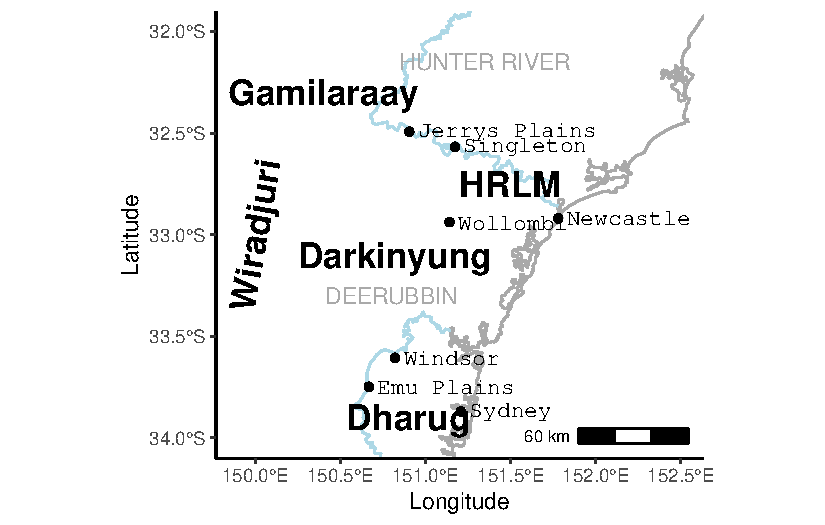
\includegraphics{harpur-dunlop-wulatji_files/figure-pdf/fig-map-1.pdf}

}

\caption{\label{fig-map}Deerubbin and the Hunter in the 1840s,
indicating languages, settlements and rivers mentioned in the text.
Sources: \citet{geoscience_australia_geodata_2003}; Nominatim;
\citet{lissarrague_salvage_2006}; \citet{lissarrague_gamilaraay_2003};
\citet{jones_darkinyung_2008}; Austlang.}

\end{figure}%

\textsubscript{Source:
\href{https://michaelgfalk.github.io/harpur-dunlop-wulatji/harpur-dunlop-wulatji.qmd.html}{Article
Notebook}}

My comparison of Harpur and Dunlop has two aims. The first aim is to
contrast Dunlop's and Harpur's poetics: I argue that Dunlop is a
\emph{universalist}, while Harpur is a \emph{particularist}. The second
aim is to clarify the problem of \emph{linguistic representation}---or
more verbosely, the \emph{literary representation of Indigenous
languages}.

Both Dunlop and Harpur represent Indigenous language for humanitarian
ends. Although Dunlop was highly sensitive to the differences between
people, her ``sentimental'' poetics relies on the universality of human
feelings to justify the universality of human rights
\citep{rudy_beyond_2021}. Thus she attempts to demonstrate the
universality of the poetic impulse by transcribing and translating a
sample of Awabakal poetry. By contrast, Harpur attempts to do justice to
Indigenous ecopoetics by drawing a link between the euphony of
particular Indigenous words and the ecological knowledge of particular
Indigenous people. Dunlop's universalism and Harpur's particularism have
both been subject to scholarly critique, but have never been compared. I
perform the comparison in sections
\hyperref[eliza-hamilton-dunlop-universalism]{2} and
\hyperref[charles-harpur-particularism]{3}.

Dunlop and Harpur also raise the broader question of how to represent a
language. Both Harpur and Dunlop wish to represent Indigenous languages
as \emph{poetic}, but they do so in different ways. Dunlop produces a
\emph{transcription}, \emph{translation} and \emph{glossary}; Harpur
produces \emph{words} and \emph{philological footnotes} embedded in an
original poem. These different forms of representation convey different
ideas about the nature of Indigenous language. Dunlop presents Wulatji's
language (the Hunter River Lake Macquarie language, or HRLM), as
\emph{syntactic} and \emph{literary.} Harpur presents the various
languages of his poem, namely Darkinyung, Gamilaraay and HRLM, as
\emph{verbal} and \emph{oral}. Despite these differences, Dunlop and
Harpur draw on a similar stock of ideas about human language, rooted in
the empiricist linguistics that then reigned in the English-speaking
world. I demonstrate this shared background in
\hyperref[linguistic-representation-and-the-conquest-of-space]{section
4}.

\subsection{Eliza Hamilton Dunlop:
Universalism}\label{eliza-hamilton-dunlop-universalism}

\begin{quote}
Since morning stars first sang in prayerful praise,\\
Since Adam's hymns resounded over space,\\
Or Sinai's hill trembled in glory's blaze;\\
Immortal song hath had acknowledged place. \citep[ll.
1-4]{dunlop_poesy_1872}
\end{quote}

For Dunlop, ``song'' is a universal feature of human nature. In the
opening lines of ``Poesy,'' she hears song in three places: in nature
(the ``morning stars''), in oral tradition (``Adam's hymns''), and in
written literature (``On Sinai's hill,'' where Moses receives the tables
of the law). In all these places, the same force of ``song'' is heard.
At all \emph{times}, too, this ``song'' is heard, for it is
``Immortal.'' Song is immortal and ubiquitous, Dunlop continues, because
it is an ``Essence inherent of the sentient mind'' \citep[l.
5]{dunlop_poesy_1872}.\footnote{In another poem of the same year, she
  extols the universality of ``IMPERIAL MIND!'', which compels
  ``Obedience'' throughout its ``boundless realm''
  \citeyearpar{dunlop_mind_1872}.} Always and everywhere, humans are
poets.

Dunlop's belief in the universality of song had deep ethical and
intellectual roots. She was a ``sentimentalist,'' whose poetry teaches
that ``the emotional experiences of others are similar to our own''
\citep[91]{rudy_beyond_2021}. She was an ``internationalist,'' whose
poetry describes the struggle for freedom among all the oppressed
peoples of the British Empire
\citetext{\citealp[60]{wu_morning_2021}; \citealp[9]{johnston_proud_2021}}.
She was a polyglot, whose poems speak in many tongues
\citep[158-159]{wafer_unmapping_2021}. Thus she expressed her
humanitarian ideals in the rhetoric, content and vocabulary of her
poetry.

As \citet{rudy_beyond_2021} insists, Dunlop's universalism was not
naive. She grew up in Ireland in the wake of the United Irish uprising
and the abolition of the Irish parliament. She visited India, where she
befriended her ``half-caste'' sisters.\footnote{Her brothers were not so
  friendly. They refused to acknowledge their Indian half-sisters, and
  denied them their inheritance
  \citetext{\citealp[39]{johnston_poetry_2021}; \citealp[63]{wu_morning_2021}}}
She settled in Australia, where she displayed an exceptional facility
for Indigenous languages, particularly their phonetics
\citep[46]{johnston_poetry_2021}, and where she campaigned publicly for
the rights of Indigenous Australians. In all these places, she was
sensitive to local conditions. She published some 100 poems in Irish and
Australian newspapers; when she did so, she chose her words carefully
for local readers, especially when republishing Irish works in Australia
\citep[94]{rudy_beyond_2021}. Her universalism was modulated by her
pragmatic sense of audience.

It is in this context that we should understand her transcription and
translation of Wulatji's poetry. The transcription is short enough to
quote in full. Its language is Awabakal, recognised today as a variety
of the Hunter River Lake Macquarie language (HRLM):

\begin{quote}
Nung-Ngnun\\
Nge a runba wonung bulkirra umbilinto bulwarra;\\
Pital burra kultan wirripang bunto\\
\strut \\
Nung-Ngnun\\
Nge a runba turrama berrambo, burra kilkoa:\\
Kurri wi, raratoa yella walliko,\\
Yulo Moane, woinya, birung poro bulliko{[}.{]}\\
\strut \\
Nung-Ngnun\\
Nge a runba kan wullung, Makora, kokein,\\
Mip-pa-rai, kekul, wimbi murr ring kirrika:\\
Nge a runba mura ke-en kulbun kulbun murrung.
\citep{wulatji_native_1848}
\end{quote}

It is difficult to say what precisely this is a transcription \emph{of}.
\citet[92]{oleary_giving_2004} argues from manuscript evidence that
Dunlop fashioned a single poem from ``three short songs'' by Wulatji. In
a manuscript she prepared in the 1870s, she does indeed label the three
sections ``Song 1,'' ``Song 2'' and ``Song 3'' \citetext{\citealp[image
60]{dunlop_vase_nodate}; \citealp[printed
in][194]{dunlop_selection_2021}}. In both the published version and the
manuscript, she gives each section the heading ``Nung-Ngung''
(\emph{nannguyn}, ``song''). Despite this evidence,
\citet{wafer_ghost-writing_2017} argues that Wulatji's poetry should
actually be seen as four ``verses'' of two lines each. He gives two
arguments: the four-verse interpretation makes the poetry more
metrically consistent \citeyearpar[204]{wafer_ghost-writing_2017}; and
the textual evidence cannot be trusted, because there is no record of
Dunlop and Wulatji's conversations
\citeyearpar[202]{wafer_ghost-writing_2017}. Did Wulatji produce one or
more discrete texts at Dunlop's request, knowing they might be
published? Did he perform at a ceremony or gathering that Dunlop
observed? Did he produce a series of verse-examples to try and teach her
about Awabakal versification? Did he improvise a performance to impress
her?\footnote{According to Threlkeld, Wulatji was a popular guest, whose
  humourous `gibes' and `song and dance' routines were highly
  appreciated by Indigenous people throughout the region \citep[quoted
  in][200]{wafer_ghost-writing_2017}.} Dunlop herself provides evidence
that it may be foolish to precisely number the poems in Wulatji's text.
In the manuscript version of the poem, she notes that Indigenous songs
are short and ``often repeated in a variety of cadence''
\citeyearpar[194]{dunlop_selection_2021}. How many different verses
would a poet like Wulatji ``repeat'' in a single performance? It is not
necessarily the case that his poetry could be neatly divided into
discrete ``poems'' independent of one another.

Dunlop preserves this ambiguity in her transcription and translation.
Her title, ``Native Poetry,'' does not specify the number of poems. When
she adapted her translation into an original song for Isaac Nathan, she
used a similarly indeterminate title, ``Pialla Wollombi,'' which she
glosses as ``the poetry or language of Wollombi''
\citep{dunlop_pialla_1848}. All this is to suggest that Dunlop does not
transcribe a \emph{text}, but rather a \emph{corpus} of Awabakal verse.
She provides the reader a sample of Wulatji's poetry, and shapes it into
a single translation for readerly consumption---for the
\emph{translation}, unlike the transcription, certainly comprises a
single text:

\begin{quote}
Our home is the gibber-gunyah,\\
Where hill joins hill on high;\\
Where the turruma and berrambo,\\
Like sleeping serpents lie;\\
And the rushing of wings, as the wangas pass,\\
Sweeps the wallaby's print from the glistening grass.\\
\strut \\
Ours are the makoro gliding,\\
Deep in the shady pool;\\
For our spear is sure, and the prey secure\ldots{}\\
Kanin, or the bright gherool.\\
Our lubras sleep by the bato clear,\\
That the Amygest's track hath never been near.\\
\strut \\
Ours is the koolema flowing\\
With precious kirrika stored;\\
For fleet the foot, and keen the eye,\\
That seeks the nukkung's hoard;\\
And the glances are bright, and the footsteps are free,\\
When we dance in the shade of the karakon tree.
\end{quote}

There are many remarkable features of this translation, but for our
purposes, the most important aspect is its vocabulary
(Table~\ref{tbl-dunlop-lang}). Dunlop includes 15 Indigenous words in
her translation. Five of these had already been incorporated into
Australian English by 1848: ``gibber-gunyah,'' ``wallaby,'' ``wanga,''
``lubra'', and probably ``koolema'' \citep{dixon_australian_2006}. She
nonetheless includes two of them---``gibber-gunyah'' and ``wanga''---in
the poem's Glossary. The other 10 words probably appear here in English
verse for the first time, and probably all originate in Wulatji's speech
(``gherool'' and ``Amygest'' being the difficult cases).

\begin{longtable}[]{@{}
  >{\raggedright\arraybackslash}p{(\columnwidth - 8\tabcolsep) * \real{0.0963}}
  >{\raggedright\arraybackslash}p{(\columnwidth - 8\tabcolsep) * \real{0.0688}}
  >{\raggedright\arraybackslash}p{(\columnwidth - 8\tabcolsep) * \real{0.0917}}
  >{\raggedright\arraybackslash}p{(\columnwidth - 8\tabcolsep) * \real{0.3349}}
  >{\raggedright\arraybackslash}p{(\columnwidth - 8\tabcolsep) * \real{0.4083}}@{}}

\caption{\label{tbl-dunlop-lang}Indigenous vocabulary in Dunlop's
translation of Wulatji. Sources: \citet{wafer_ghost-writing_2017}; HRLM
\citep{lissarrague_salvage_2006}; Darkinyung
\citep{jones_darkinyung_2008}; Gamilaraay
\citep{lissarrague_gamilaraay_2003}; Sydney \citep{troy_sydney_1993};
\citet{dixon_australian_2006}}

\tabularnewline

\toprule\noalign{}
\begin{minipage}[b]{\linewidth}\raggedright
Dunlop's translation
\end{minipage} & \begin{minipage}[b]{\linewidth}\raggedright
Wulatji's text
\end{minipage} & \begin{minipage}[b]{\linewidth}\raggedright
Dunlop's definition
\end{minipage} & \begin{minipage}[b]{\linewidth}\raggedright
HRLM equivalents
\end{minipage} & \begin{minipage}[b]{\linewidth}\raggedright
Other equivalents
\end{minipage} \\
\midrule\noalign{}
\endhead
\bottomrule\noalign{}
\endlastfoot
gibber-gunyah & & Cave in the rock & kuyung \textasciitilde{} kuyang
\emph{camp, camp fire; also town} & giba \emph{stone or rock}, gunya
\emph{hut} (Sydney) \\
turruma & turrama & War arms & TaRama \emph{war boomerang} & \\
berrambo & berrambo & War arms & pirampu \emph{waddy; club (Wafer)} & \\
wanga & & A species of pigeon & & wungawunga \emph{Wonga pigeon}
(Sydney); wangawanga \emph{Wonga pigeon} (Darkinyung) \\
wallaby & buntoa & & walapi \textasciitilde{} walapay \emph{wallaby};
paNTarr \emph{kangaroo} & wulaba \emph{rock wallaby} (Sydney) \\
makoro & Makoro & Fish & makurr \emph{fish} & magura \emph{fish}
(Sydney) \\
kanim & & Eel & kaNiyn \textasciitilde{} KaNang \emph{freshwater eel}
& \\
gherool & & Mullet & & djirul \emph{mullet} (Darkinyung) \\
lubra & mura ke-en & & marr{[}a{]}kiyn \emph{young maiden, woman, girl}
& {[}The etymology of \emph{lubra} is unknown; possibly from a Tasmanian
language{]} (Dixon et al) \\
bato & kokein & Water & paTu, kukuyn \emph{fresh water} & \\
Amygest & & White fellow & & \\
koolema & wimbi & & wimpi \emph{vessel made from the knots of trees and
used as baskets or bowls} & guliman \emph{coolamon} (Gamilaraay) \\
kirrika & kirrika & Honey & kiR{[}i{]}ka \emph{white honey} & \\
nukkung & & Wild bee & Nakang \emph{native bee} & \\
karakun & & Oak Tree & karakaNpa \emph{place of swamp-oaks} & \\

\end{longtable}

\textsubscript{Source:
\href{https://michaelgfalk.github.io/harpur-dunlop-wulatji/harpur-dunlop-wulatji.qmd.html}{Article
Notebook}}

What is remarkable is the relationship between Dunlop's words and
Wulatji's. We might expect Dunlop only to introduce Indigenous words in
her poem if they are present in Wulatji's text, or common in Australian
English. But this is not her practice. In just four cases, Dunlop
incorporates a word from Wulatji's text into her translation:
``turruma'', ``berrambo'', ``makoro'' and ``kirrika.'' In the other
cases, she either inserts a new word into the poem (e.g.~``wanga,''
``nukkung'') or translates one of Wulatji's words by a \emph{different}
Indigenous word (e.g.~``kokein'' → ``bato'', ``wimbi'' → ``koolema'').
Her translation ultimately incorporates vocabulary from at least three
or four Australian languages, but in neither the text nor the Glossary
does she indicate which languages they are. Dunlop effectively develops
her own poetic language, combining English, Wulatji's own speech, and
the speech of other Indigenous peoples across Eastern NSW. She confers
unity on Wulatji's verses, combining them into a single poem, and she
confers unity on the languages of the colony, combining them into a
single tongue. How should we interpret this unity?

Dunlop's translation is a representation of Indigenous speech. Thus it
has two interlinked aims: it must capture the lyrical qualities of
Wulatji's verse; and it must signal its Indigenous Australian origin to
the reader. In this light, the inclusion of familiar words such as
``gibber-gunyah'' and ``wallaby'' makes sense. These words signal to the
reader that this is an ``Australian'' poem. The choice to translate
Wulatji's words by other words sometimes serves this purpose of
familiarisation (e.g.~``mura ke-en'' → ``lubra''), and sometimes seems
to be an aesthetic decision: e.g.~Dunlop presumably found ``bato clear''
more euphonious than ``kokein clear'' or alternative phrasings. The
poem's rhyme and metre also serve these dual purposes of familiarisation
and exoticism. The rhymes follow the familiar scheme of \emph{Venus and
Adonis} (\emph{ababcc}). Meanwhile the accentual metre emulates the old
ballads that represented ``tradition'' for Romantic readers: The number
of beats follows a fixed pattern in each stanza (3-3-4-3-4-4), while the
rhythm shifts freely between binary and ternary. In sum, Dunlop presents
Wulatji's poetry as though it is an ancient ballad in an ``invented
tradition'' of Australian verse, the kind of poem you might encounter in
Thomas Percy's \emph{Reliques of Ancient English Poetry} (1775) or
Walter Scott's \emph{Minstrelsy of the Scottish Border} (1802).

To turn Wulatji's poem into a ``Relique'' of Australian verse, Dunlop
amplifies the text. Wulatji's original text is not remotely ballad-like.
It has a terseness that bespeaks its rich metaphysical background.
\citet[206]{wafer_ghost-writing_2017} translates the first verse thus:

\begin{quote}
Ours is the place where the mountains cohabit with the heights\\
The eaglehawks and wallabies are happy
\end{quote}

When she chooses, Dunlop captures the literal sense of Wulatji's verse
well, e.g.~``wonung bulkirra umbilinto bulwarra'' → ``where hill joins
hill on high.'' But she generally amplifies the verse to conform with
European expectations of the lyric. Human embodiment is implicit in
Wulatji's poem. Dunlop makes it explicit, indicating that the mountains
are Wulatji's ``home.'' The senses are muted in Wulatji's poem. Dunlop
invokes the senses, so that the birds have ``rushing wings,'' and the
wallabies play on the ``glistening grass.'' She also, inexplicably,
turns Wulatji's ``wirripang'' (``eaglehawk'') into a Wonga pigeon. These
amplifications are typical of Dunlop's translation. She inserts
individual persons into the poem, placing their bodies in the landscape
and invoking their sensory experiences of nature.

Dunlop thus presents Wulatji's verse as \emph{syntactic} and
\emph{literary}. It is not the individual words of his poetry that
matter, but their connection into smoothly-flowing verse. And though
Wulatji's verse is oral rather than written, Dunlop presents it as
implictly literary, like the ancient ``Reliques'' of English verse
preserved in book and manuscript. Dunlop emphasises the syntax and
literacy of Wulatji's verse in her introduction to the poem:

\begin{quote}
There is a god of Poesy, Wallatu, who composes music, and who, without
temple, shrine, or statue, is as universally acknowledged as if his
oracles were breathed by Belus or Osiris: he comes in dreams, and
transports the individual to some sunny hill, where he is inspired with
the supernatural gift. \citep{wulatji_native_1848}
\end{quote}

Wulatji's poetry is syntactic because it does not comprise individual
words. Instead it comes complete, in the form of ``oracles'' delivered
by divine inspiration. Wulatji's poetry is literary because the god of
his inspiration, Wallatu, is the same in kind as the gods of the Celts
(Belus) and Egyptians (Osiris), whose writings lie at the origins of
Western civilisation.\footnote{On the coincidence between Wulatji's name
  and Wallatu's, see \citet[91]{oleary_giving_2004} and
  \citet[199]{wafer_ghost-writing_2017}.} Dunlop the Irish writer
recognises in Wulatji a fellow Celt. And this is unsurprising, because
``Poesy'' is universal, and can be recognised as easily in Australia as
anywhere else. Thus the freedom of Dunlop's translation. She does not
translate the literal sense of the words, but communicates the ``Poesy''
that inspires them.

\subsection{Charles Harpur:
Particularism}\label{charles-harpur-particularism}

\begin{quote}
A thousand bright particulars are given,\\
And they outshine the very stars of heaven! (``Ideality'', h185b)
\end{quote}

Harpur's poem is on a grander scale than Dunlop's. \emph{The Kangaroo
Hunt, or A Morning in the Mountains: A Descriptive Poem in Six Parts: By
Charles Harpur. An Australian} is a long and ambitious work that has
been described as ``Australia's first epic poem''
\citep[81]{gelder_colonial_2020}. It describes an ``idealised'' kangaroo
hunt that lasts from sunrise to sunset. As the youthful party of white
hunters harry the kangaroo, Harpur describes the sights and sounds of
the Australian bush, expanding on the verse in detailed footnotes. The
poem pulls in two directions. In one direction, Harpur seeks to
``idealise'' the hunt, blending the details of many possible hunts into
``one Eden-piece embathed with a luminous atmosphere of sentiment''
(h209-af). In another direction, Harpur seeks to capture specific
details of land and language, to capture the particular qualities of
each bird, tree, geological feature---or Indigenous word. We will see
that in his hunt for particularity, Harpur presents Indigenous languages
as primarily \emph{oral} and \emph{verbal}. A language comprises words
that are spoken by particular people in particular places.

Harpur uses 12 Indigenous words in either the body of the poem or its
footnotes (Table~\ref{tbl-harpur-lang}).\footnote{I am indebted to Jim
  Wafer for sharing his notes on Harpur's Indigenous vocabulary, which
  helped especially with the difficult \emph{teleltella}.} Generally
speaking, Harpur's transcriptions are sound, and it is not difficult to
look up the words in a modern dictionary. It is nonetheless difficult to
identify the languages of Harpur's poem, for two main reasons. The first
reason is lack of biographical evidence. Harpur does not name his
informants, nor does he describe precisely where he encountered them.
The only geographic detail he provides is in his footnote on the words
``jimbuc'' and ``whirring'', which I discuss below. The second reason
lies in the textual record. Harpur began the poem in the 1840s, while
living on the Hunter, and completed it in the 1860s, while living in
Eurobodalla. With the exception of a single extract published in the
\emph{Weekly Register} in 1843, all the surviving versions of the poem
date to the 1860s \citep{harpur_australian_1843}. Only \emph{one}
Indigenous word, ``duaralli,'' appears in the 1843 newspaper extract.
When did Harpur learn and insert the other words? Despite these
problems, it is possible to find all but one of Harpur's words in modern
dictionaries.

\begin{longtable}[]{@{}
  >{\raggedright\arraybackslash}p{(\columnwidth - 12\tabcolsep) * \real{0.0479}}
  >{\raggedright\arraybackslash}p{(\columnwidth - 12\tabcolsep) * \real{0.4110}}
  >{\raggedright\arraybackslash}p{(\columnwidth - 12\tabcolsep) * \real{0.0890}}
  >{\raggedright\arraybackslash}p{(\columnwidth - 12\tabcolsep) * \real{0.0959}}
  >{\raggedright\arraybackslash}p{(\columnwidth - 12\tabcolsep) * \real{0.1438}}
  >{\raggedright\arraybackslash}p{(\columnwidth - 12\tabcolsep) * \real{0.0651}}
  >{\raggedright\arraybackslash}p{(\columnwidth - 12\tabcolsep) * \real{0.1473}}@{}}

\caption{\label{tbl-harpur-lang}Indigenous Vocabulary in \emph{The
Kangaroo Hunt}. Sources: Darkinyung \citep{jones_darkinyung_2008}; HRLM
\citep{lissarrague_salvage_2006}; Gamilaraay
\citep{lissarrague_gamilaraay_2003}; Wiradjuri \citep{grant_new_2010};
Dhurga \citep{ellis_dhurga_2020}; Sydney \citep{troy_sydney_1993}; also
Jim Wafer, personal communication.}

\tabularnewline

\toprule\noalign{}
\begin{minipage}[b]{\linewidth}\raggedright
Harpur's word
\end{minipage} & \begin{minipage}[b]{\linewidth}\raggedright
Harpur's definition
\end{minipage} & \begin{minipage}[b]{\linewidth}\raggedright
Referent
\end{minipage} & \begin{minipage}[b]{\linewidth}\raggedright
Darkinyung
\end{minipage} & \begin{minipage}[b]{\linewidth}\raggedright
HRLM
\end{minipage} & \begin{minipage}[b]{\linewidth}\raggedright
Gamilaraay
\end{minipage} & \begin{minipage}[b]{\linewidth}\raggedright
Other
\end{minipage} \\
\midrule\noalign{}
\endhead
\bottomrule\noalign{}
\endlastfoot
Euroka & ``an aboriginal name of the sun'' & the sun & & panyal & yaraay
& yurraga (Wiradjuri); yuraga (Dhurga) \\
bidawong & ``flying squirrel'' & glider & & pitjang & bagu & budha-rang
(Wiradjuri) \\
kindyne & ``ring-tailed possum'' & ring-tailed possum & \textbf{gindang}
& wilay \emph{possum} & garrawir & \\
gooburra & ``the large kind of king-fisher which is commonly known by
the tasteful and poetic sobriquet of the Laughing Jackass'' & kookaburra
& & \textbf{kukaparr} & gugurrgaagaa & gugubarra (Wiradjuri) \\
teleltella & ``a large and solitary kind of bell-bird'' & crested
bellbird & & & banbandhuluwi & dilbanyi \emph{ring--to ring as a bell}
(Sydney) \\
warragl & ``an aboriginal name of the native dog'' & wild dog & miri
\emph{dog, wild dog} & \textbf{waRikal} & & wuragal (Sydney) \\
yerowala & ``blue-mountain parrot'' & rainbow lorikeet &
\textbf{wagarala} \emph{parrot} & wakalarr \textasciitilde{} wakilarr
\emph{red parrot; rosella} & & wiragala \emph{australian ringneck}
(Wiradjuri) \\
duaralli & ``the kangaroo-rat;'' attributed to ``the blacks of the
Hunter'' in 1843, but to ``blacks of the interior'' in 1867 (h209-df) &
eastern bettong & dhurawayi & & \textbf{dhurrawaay} & \\
maroo & ``a sort of brush iron-wood'' & ?grey box & & \textbf{maru}
\emph{thorny bush} & & \\
wallaroo & ``wallaroo''; ``the male \ldots{} {[}is{]} almost black, and
the female \ldots{} {[}is{]} a sort of cream color'' & eastern wallaroo
& \textbf{walaru} \emph{black kangaroo} & & yulama & wularu (Sydney) \\
jimbuc & ``a little shag-haired species of kangaroo;'' metaphorically,
``sheep'' & brush-tailed rock wallaby & & & \textbf{dhimba} \emph{sheep}
& \\
whirring & name for ``jimbuck'' among the people of ``the Hawksbury
mountains'' & brush-tailed rock wallaby & \textbf{wirayn} & wayiring
\emph{wallaby} & wan.guy & wirrang (Wiradjuri) \\

\end{longtable}

\textsubscript{Source:
\href{https://michaelgfalk.github.io/harpur-dunlop-wulatji/harpur-dunlop-wulatji.qmd.html}{Article
Notebook}}

The linguistic evidence suggests that the language of the poem is
primarily Darkinyung, HRLM and Gamilaraay. This finding is consistent
with the one biographical clue that Harpur provides in the poem. The
clue lies in the word ``jimbuc,'' which Harpur attributes to the
``Blacks of the Hunter,'' as opposed to the ``blacks of the Hawksbury
mountains:''

\begin{quote}
Jimbuc is an aboriginal name of little shag-haired species of kangaroo
which is peculiar to mountain copses. It may be called the mountain
wallaby, being in relation to the wallaroo what the common wallaby is to
the kangaroo proper. The jimbuc is the least elegant in its form, and
the dullest in its nature, of all the kangaroo kinds---of all such at
least as I happen to be acquainted with. The Blacks of the Hunter call
the sheep jimbuc, no doubt from a resemblance, however remote, arising
out of the hairy shagginess of the one and the woolliness of the other.
But this, like most other of our indigenous animals, is named variously
by the aboriginal tribes of different localities: and is (or was) known
amongst the Hawksbury mountains by the native name of \emph{whirring}.
(h209-gf)
\end{quote}

By the ``Hawksbury mountains,'' Harpur presumably refers to the rocky
highlands that lie between Deebrubbin and the Hunter Valley. If this is
so, then the language he would most likely encounter in that region is
Darkinyung. The first road between Sydney and the Hunter Valley ran
through this region Harpur calls the ``Hawksbury mountains,'' so Harpur
is likely to have traversed the region numerous times when moving
between the Hunter, Deerubbin and Sydney.

The case for ``the Blacks of the Hunter'' is more difficult. In the
1840s and 50s, Harpur spent most of his time moving around Singleton and
Jerrys Plains. According to \citet[13]{lissarrague_salvage_2006}, this
was a bilingual zone. Towards the east, the Wonnarua and Geawagal spoke
varieties of HRLM, Wulatji's tongue. Towards the west, the people spoke
another language, and the available sources are unclear what it was.
Lissarrague suspects it was either Gamilaraay or Darkinyung. Since
Darkinyung is the most likely candidate for Harpur's language of the
``Hawksbury mountains,'' his language of the ``Hunter'' is more likely
to be Gamilaraay. This is broadly consistent with
Table~\ref{tbl-harpur-lang}, which shows that there is a compelling
Darkinyung, HRLM, or Gamilaraay equivalent for nine of Harpur's 12
Indigenous words (marked in bold).

The example of ``jimbuc'' supports this general picture. Today,
\emph{jumbuck} is cherished by settler Australians as a slang word for
sheep, immortalised in the popular song \emph{Waltzing Matilda}.
\citet[56]{dixon_australian_2006} suggest that the word may derive from
English \emph{jump}, or perhaps from the Gamilaraay word \emph{dhimba},
but admit that neither hypothesis can be ``confirmed.'' Harpur's
footnote provides concerete support for the hypothesis that
\emph{jumbuck} derives from Gamilaraay \emph{dhimba}. The hypothesis
gains strength given the specificity of Harpur's description: Harpur
insists that the word referred specifically to the ``mountain wallaby,''
which from his description is clearly the brush-tailed rock wallaby
(\emph{Petrogale penicillata}). The compilers of the modern
\emph{Gamilaraay-Yuwalaraay-Yuwaalayaay} dictionary were unable to find
a word specifically for the brush-tailed-rock wallaby, and record the
word \emph{dhimba} solely in its meaning of \emph{sheep}
\citep[62]{lissarrague_gamilaraay_2003}. If we can trust Harpur's
testimony on this point, then the old riddle of \emph{jumbuck} is
solved, and we can be surer that some of Harpur's informants in the
Hunter spoke Gamilaraay.

Although it seems certain that Harpur learned most of the words directly
from Darkinyung, Gamilaraay and HRLM speakers, some of the words present
problems. It is of course quite probable that Harpur learned the words
``wallaroo,'' ``gooburra'' and ``warragl'' simply by learning English:
these words had passed into Australian English from Wiradjuri and the
Sydney language by the 1830s \citep{dixon_australian_2006}. The real
problem words are ``Euroka,'' ``bidawong'' and ``teleltella.''

The origin of ``teleltella'' is most obscure. Wafer (personal
communication) suggests that \emph{dilbanyi}, a word in the Sydney
Language, could be a possible source. Gamilaraay \emph{banbandhuluwi}
has a promising number of syllables and the correct meaning, but the
vowels and consonants differ considerably from Harpur's transcription.
It is possible that ``teleltella'' represents a hitherto unattested
Darkinyung or HRLM word: no word for ``crested bellbird'' appears in
either dictionary.

The other problem words, ``bidawong'' and ``Euroka,'' are attested in
Wiradjuri, a language spoken in regions bordering Darkinyung, HRLM and
Gamilaraay. ``Euroka'' is also attested in Dhurga, the local language of
the south coast where Harpur was living in the 1860s. The data suggest
three hypotheses: (1) Harpur had Wiradjuri informants; (2) ``bidawong''
and/or ``Euroka'' were present in Darkinyung but are hitherto
unattested; (3) Harpur inserted the word ``Euroka'' into the poem after
he learned it from Dhurga speakers in the 1860s. If hypothesis (1) is
true, it would suggest that the area west of Singleton may have been
trilingual, with speakers of Wiradjuri, HRLM and Gamilaraay all
frequently present. If hypotheses (2) and/or (3) are true, this would be
consistent with Lissarrague's surmise that the area west of Singleton
was a transitional zone between HRLM and Gamilaraay. These hypotheses
are hard to adjudicate, given the lack of corroborating evidence, but
all are consistent with the general impression that Harpur learned most
of his Indigenous vocabulary directly from local Indigenous informants
in the 1830s and 40s.

While the \emph{facts} of the case are murky, the \emph{poetics} are
clear. In sharp distinction to Dunlop, Harpur presents each word as a
particular word spoken by particular people in a particular place.
``Jimbuc'' and ``whirring'' are only the most obvious instances.
Consider these lines from Part II, when Harpur describes the sunrise:

\begin{quote}
Uncovered no longer the forest dog prowls,\\
Though so bold in the dark;\\
And the kindynef and bidawongg haste to their holes\\
In the spouts of yon old ironbark:\\
While on its one bare blasted limb\\
The gooburrah sits in the fog-wreath dim,\\
Glorying loud with a laughter-like glee\\
In the march of the dayspring's victory {[}\ldots{]} (h209-cf)
\end{quote}

In each footnote, Harpur identifies the word as ``an Aboriginal name'',
emphasising the indefinite article in footnote \emph{g}: ``I say
\emph{an} aboriginal name, because almost every tribe of Blacks has a
different set of names for our indiginous animals.'' (h209-cf) His
precision about language is linked to his precision about nature. He
places each animal in its ecological niche: the dog's hunting patterns
change in the daytime, the ``bidawong'' (glider) and ``kindyne''
(ring-tailed possum) nest specifically in the ``ironbark,'' and the
kookaburra sits on a ``bare'' branch where it can see its prey.
\citet[322]{dixon_charles_1980} compares the poem to a ``natural history
painting,'' which presents a ``typical and comprehensive cross section
of the forest environment.'' Natural history provides a ground-truth for
Harpur's analysis of names. Each animal or plant can be classified by
species, then an appropriate name for the species can be selected from
colonial English or local Indigenous languages. In one case, Harpur
invents his \emph{own} word for a species, having failed to locate an
appropriate name. His invented name for the eastern whip-bird, ``Jehu,''
alludes to the bird's colonial nickname of ``coachman's whip'' (h209-gf,
note d).\footnote{Harpur's name never caught on, although Henry Kendall
  borrowed it for his own kangaroo hunt poem. Kendall was apparently
  unaware the ``Jehu'' is a colloquial term for a coachman, and changed
  the spelling to ``echu,'' emphasising its onomatopoeia
  \citep[73]{gelder_colonial_2020}.}

Harpur chooses Indigenous names because they are more ``poetic.'' For
instance, to justify the choice of ``gooburra'' as a name for the
kookaburra, he sarcastically dismisses the ``the tasteful and poetic
sobriquet of the Laughing Jackass'' conferred on the bird by white
settlers (h209-cf). His discussion of Indigenous names is most pregnant
in the case of ``Euroka,'' which he invokes in Part I of the poem:

\begin{quote}
Or while Eurokab first displays\\
His burning rim on the ancient hill,\\
{[}\ldots{]}\\
He floods abroad his golden light\\
In one unbroken mass immense\\
Of life-essential influence {[}\ldots{]}\\
\strut \\
b Euroka is an aboriginal name of the sun. It is at once euphonious and
robust, and has therefore a certain sounding adequacy as a vocable, and
thence somewhat of ideal unison with the golden progression and godlike
port of that paramount luminary. (h209-bf)
\end{quote}

Harpur makes two claims for ``Euroka.'' First, the word itself is
``euphonious and robust'' as a ``vocable.'' Second, the word's euphony
means it can achieve an ``ideal unison'' with the reality it
denotes---namely, the sun. For Harpur, the ``ideality'' of poetry arises
from the unification of word and world.\footnote{The word is Harpur's.
  See for instance h185b.} To idealise the world, the poet must see each
particular thing correctly, and then the select the word that will
communicate that particularity. Harpur thus makes a strong claim for
Indigenous poetics. Twelve times in \emph{The Kangaroo Hunt}, Harpur
claims that Indigenous people have properly seen the world, and found
the ideal word to communicate what they have seen
\citep[5]{webby_representations_2013}. In the case of Euroka, Harpur
emphasises the point by using Euroka himself as a symbol of ideality.
Euroka illuminates the earth, uniting all things in the ``one unbroken
mass'' of his ``life-essential influence.''

Harpur observes Euroka rise, but does not actually invoke him as the
muse. Instead, Harpur compares himself to Euroka: as Euroka rises to
illuminate the world, so the poet walks to the top of a hill to survey
the scene. At this point in the poem, its troubling colonial elements
come into view:

\begin{quote}
While thus Euroka riseth red,\\
Up, even to the kingly head\\
Of some proud eminence, we climb,\\
Where high amid the crags sublime,\\
Australia's yet unchristened Muse,\\
A wandering Spirit of beauty rare,\\
Loves oft to gem her streaming hair\\
With heaven's selectest dews,\\
And scarf her bosom bright and bare\\
With a robe of Morning richest hues;\\
Giving the while to all objects there,\\
All sounds,---the water drip just heard---\\
The hum of insect---voice of bird,---\\
To every echo and every air\\
A poetry unfelt elsewhere. (h209-bf)
\end{quote}

In this image, Harpur illuminates the world with the ideal beauty of
poetry, just as Euroka illuminates the world with his light. But the
introduction of ``Australia's yet unchristened Muse'' complicates
things. What does ``unchristened'' mean? Does it mean that the Muse is
unnamed, or simply that she has not ``yet'' been named by the Christian
settlers? In either case, what is the significance of her naming? Harpur
defends Indigenous speech as ``euphonious'' and ``poetic.'' He suggests
that the poetry of the forest can be seen in the ``dew,'' heard in ``All
sounds,'' and ``felt'' in the air. He suggests that the Muse is
solar-powered, as Euroka ``robes'' her in beauty. Harpur himself
refrains from naming the Muse in this very poem where he foreshadows her
``christening.'' Does all this mean that the Muse of Australia is
eternal, and freely available to any human being to happens to walk in
her domain? Or, more darkly, does Harpur propose that the white settlers
will one day expropriate the Muse from the first Australians, by
``christening'' her? Harpur does not resolve these issues. \emph{The
Kangaroo Hunt} is a poem of futurity, and Harpur looks forward to a time
when the poem's own questions may be answered.

In the final lines of the poem, however, Harpur does recur to the Muse.
In these lines, Harpur describes himself as an ``uncouth'' poet, and
apologises for his lack of education. He then aligns his own
``uncouthness'' with the ``virginity'' of the Muse:

\begin{quote}
Thus nurtured,---self urged, first he knew\\
Australia's virgin Muse to woo,\\
And of Song's bright mysteries 'gan to guess\\
With a lone self-cherished studiousness {[}\ldots{]} (h209-gf)
\end{quote}

Again the imagery is ambiguous. Does the virginity of the Muse imply
that one day, she will marry the white settlers? Or does it imply that
she is \emph{always} a virgin, and that the poetry of Australia truly
belongs to no-one, neither settler nor Indigenous? Harpur forecloses a
third possibility, that the Muse was already married when the white
settlers came. He is anxious to secure his poetic authority. Without the
benefit of education, he claims authority from his connection to the
land. But he realises full well that Indigenous Australians already have
this connection. In Part III, Harpur acknowledges Indigenous Australians
as ``the former lords of the soil.'' He praises their wise husbandry,
which prevented the mass ``extinction'' of native birds brought about by
white settlement (h209-df, note e). The wise husbandry and poetic speech
of Indigenous Australians are both a problem and a solution for Harpur.
Indigenous Australians have proven there is an Australian poetry
inherent in the land, but they also threaten the white settler's right
to compose that poetry. The unnamed, unmarried ``Muse of Australia'' is
Harpur's attempt to resolve this contradiction.

Where Dunlop's translation is smooth and familiar, Harpur's epic is
craggy and difficult. He enjoins the reader to pause on each word, each
image, and appreciate its robustness. Thus in the poem's \emph{language}
as well as its plot, Harpur dramatises the struggle to comprehend the
Australian environment. This struggle reflects broader themes in
Harpur's work: his struggle to cement his authority as the colony's
``first'' poet \citep{mead_charles_1990}; and his interest in the
struggle between ``nature and intellect'' in cognition
\citep[460]{ackland_charles_1983}. Harpur adopts particular Darkinyung,
Gamilaraay and HRLM words whose sound and meaning allows him to
comprehend the landscape more fully. This is why I say his
representation of Indigenous language is \emph{verbal} and
\emph{oral}---he sees language as a collection of \emph{words} that are
\emph{spoken} to denote particular things.

\subsection{Linguistic representation and the conquest of
space}\label{linguistic-representation-and-the-conquest-of-space}

Both Dunlop and Harpur claim poetic authority, and seek to write an
Australian poetry which somehow reconciles the rights of white settlers
and Indigenous Australians. In both cases, however, the white poet
asserts the right to choose: to open the pantry of Indigenous poetry,
and select the choicest morsels for their own compositions. Today this
might be condemned as cultural appropriation
\citetext{\citealp[85]{oleary_giving_2004}; \citealp[47]{johnston_poetry_2021}},
but neither Dunlop nor Harpur seem to have been concerned that
linguistic ``borrowings'' could be a kind of theft. It was simply
obvious to Harpur and Dunlop that words don't belong to anybody. Why
not? In this section, I sketch the linguistic philosphy that justified
their attitudes.

In Harpur and Dunlop's time, the empiricist philosophy of language
predominated in the English-speaking world. Dunlop was well-versed in
British empiricism, having read David Hume by the age of 12
\citep[76]{hansord_imperial_2021}. Harpur's education is not well
attested, but he was a close reader of Percy Shelley, whose debts to
radical empiricism are well known.

In the empiricist theory of language, language is made up of ``signs,''
and these ``signs'' are simply labels that we apply to objects we
perceive \citep[159]{bergheaud_empiricism_1985}. As
\citet[405]{locke_essay_1975} argues, signs are arbitrary: words become
signs for our ideas through ``voluntary imposition.'' Initially, we
label ``simple ideas,'' such as \emph{red}, \emph{wood} or \emph{water}.
Later, we stitch together simple ideas to build up ``complex ideas,''
and label these complex ideas with signs such as \emph{government} or
\emph{religion} \citeyearpar[§3.2]{locke_essay_1975}. Locke's view is
psychological and individualistic. My perceptual system delivers
sensations into my mind, and I choose to label them with other
sensations, namely sounds and visible characters, which then become
signs. Locke was accordingly sceptical of abstract concepts. Ultimately
a word is only meaningful if it can be reduced to simple, perceptible
ideas such as \emph{hard} or \emph{round}. But when we use abstract
words such as \emph{power}, it is easy to forget the complex of
particular sensations that the word refers to. Thus we often ``have very
good and approved Words in {[}our{]} Mouths, and Writings, with very
uncertain, little or no signification''
\citeyearpar[438]{locke_essay_1975}.

In Harpur and Dunlop's time, the most famous proponent of Locke's ideas
was John Horne Tooke \citep[chap.~2]{aarsleff_study_1967}.
\citet[vol.~1, p.~18]{tooke_epea_1805} begins with the proposition that
``Words are the \emph{signs} of \emph{things},'' and then poses a
difficult problem: there are many words, such as prepositions and
articles, which do not refer to perceptible things. You cannot smell
\emph{an} or touch \emph{of}. To save the empiricist theory of language,
he attempts to prove that words such as \emph{an} or \emph{of} are
``abbrevations'' of nouns and verbs, offering some very inventive
etymologies to illustrate his theory. He justifies the theory by
observing that the human mind has an innate love of ``\emph{dispatch}''
\citeyearpar[vol.~1, p.~27]{tooke_epea_1805}. We wish to speak quickly,
therefore we abbreviate, and generate all the abstract words of a fully
grammaticizised language. Tooke's ideas were later promulgated by the
utilitarians, who in turn influenced the young Tennyson and Browning
\citep[642-643]{cooper_womens_2006}. In his posthumous writings on
language, Jeremy \citet{bentham_essay_1843} argues that every ``sign''
in language stands for some ``entity,'' and distinguishes ``real'' from
``fictitious'' entities. A ``real'' entity is ``an object, the existence
of which is made known to us by one or more of our five senses''; a
``fictitious'' entity is ``an object, the existence of which is feigned
by the imagination'' \citeyearpar[325]{bentham_essay_1843}. A word
denoting a ``fictitious'' entity can only be meaningful if the
fictitious entity can be broken down into real, perceptible entities: to
every word with an ``immaterial import there belongs, or at least did
belong, a material one'' \citeyearpar[329]{bentham_essay_1843}. For
Tooke, Bentham, and their empiricist forebears, human language is
universal. Everywhere the operations of the mind are the same.
Everywhere the mind encounters the same kind of material things. Since
words are names for things, I can always understand the meaning of a
word by learning what things it refers to, even when the word seems to
denote an abstract concept.

This analysis reveals that Dunlop's universalism and Harpur's
particularism are two sides of the same coin. Harpur's particularism
would be impossible without the universality of the mind. Dunlop's
universality would be impossible without the particularity of the
senses. Harpur asserts the universality of the human mind in mystical
poems such as \emph{The Tower of the Dream} (1851-53, h642a) and
\emph{Cosmoplasticus} (1857, h696c). In the major work of his maturity,
\emph{The Witch of Hebron} (1867, h689-gd), he suggests that each person
originates alike in an ``aboriginal inception, / {[}\ldots{]} A
self-producing knot of living shoots{[}.{]}''\footnote{This image does
  suggest a ``developmental'' viewpoint that is superficially similar to
  Herder's historicism; but Harpur's view of development was more
  teleological that Herder's \citep[6-10]{falk_endless_2019}.} Thus
Harpur's particularism has a universalist substrate. By contrast,
Dunlop's universalism expresses itself in particularism. We have already
seen how she amplifies Wulatji's text with sensory images, explicitly
evoking the sounds, sights and feelings that Wulatji himself leaves
implicit. In other poems, she describes particular places in loving
detail, as in this stanza on her home at Mulla Villa:

\begin{quote}
~~~~Deep, silent water---water dark and still,\\
\strut ~~~~Bowered in the desert, lonely lot is thine!\\
\strut ~~~~For thee, no courtly Bard, essays his skill\\
At thy cool font inspired---``sweet Mulla mine.''
\citep[198]{dunlop_selection_2021}
\end{quote}

In this stanza, she evokes the sights and sounds of her home (``silent
water---water dark'') in order to particularise it: her ``Mulla,'' the
creek behind her home, is \emph{not} the ``Mulla'' where the ``courtly
bard'' Edmund Spenser lived in the sixteenth century.

Harpur is traditionally labelled ``Romantic''
\citep[e.g.~by][]{kane_australian_1996, harpur_general_1987}, while his
female contemporaries such as Dunlop are labelled ``sentimental.''
Harpur and Dunlop's shared empiricism, however, suggests that this
distinction is illusory. Like earlier Romantics, such as Samuel Taylor
Coleridge or Felicia Hemans, both Harpur and Dunlop seek the ``One
Mind'' that is immanent in experience. \citet[69]{wu_morning_2021} is
therefore quite correct when he writes: ``Dunlop realised as clearly as
any of the Romantic poets that art lives in the realm of the ideal''
\citetext{\citealp[see
also][109]{minter_settlement_2021}; \citealp[79]{hansord_imperial_2021}}.

What does Dunlop and Harpur's empiricism have to do with the ownership
of words? We can answer this question by comparing the then-dominant
English theory of language with the then-dominant German theory. In
Harpur and Dunlop's time, German scholars had rejected the tradition of
``philosophical grammar'' represented by Locke, Tooke and Bentham, and
were pursuing the new discipline of ``historical philology''
\citetext{\citealp[xii]{foucault_order_2002}; \citealp[3-6]{aarsleff_study_1967}}.
In historical philology, the sign is no longer an arbitrary label for a
sensation. Instead, words themselves are objects that have their own
histories, can they cannot simply be detached from the languages of
which they form a part. As \citet[256]{foucault_order_2002} puts it, in
historical philology, language has an ``interior `mechanism'\,'' that
determines the distribution and interrelations of words. If this is the
case, then linguistic borrowing becomes problematic. One of the early
proponents of historical philology, Johann Gottfried
\citet[38-39]{herder_against_1993} illustrates the problem:

\begin{quote}
You must first enter the spirit of a nation in order to empathize
completely with even one of its thoughts or deeds. You must discover a
characterizing word through which you can understand everything in
depth. Otherwise, you simply read a word.
\end{quote}

A word is not a name applied by an individual to a sensation; it is the
expression of the ``spirit of a nation.'' If you do not know this
``spirit,'' you do not ``understand'' the word, you simply ``read'' it.
Herder's argument invalidates Dunlop's procedure of swapping one word
for another in her translation: ``bato'' (\emph{paTu}) cannot translate
``kokein'' (\emph{kukuyn}): these are different words, even if they
refer to the same object of perception. Herder's argument also
invalidates Harpur's procedure of selecting words for their
``euphoniousness:'' Harpur has merely ``read'' the word for its sounds,
rather than grasping its spirit.

One implication of historical philology is that human nature changes.
Human nature is ``a pliant clay, which assumes different shapes under
different circumstances, needs, and burdens''
\citep[43]{herder_against_1993}. This view of human nature undermines
the metaphysical presuppositions of Harpur and Dunlop's poetry. There is
no one mind that expresses itself in song, as Dunlop believed. We do not
live in a shared world of particulars that guarantee the meaning of
words, as Harpur believed. Herder and the historicists could not endorse
Dunlop and Harpur's programme.

This analysis indicates precisely why it is anachronistic to accuse
Harpur and Dunlop of ``cultural appropriation.'' In their view, words
were labels for perceptions, and it was open to any person at any time
to invent or adopt a new label.\footnote{How Wulatji and other
  Indigenous informants viewed these linguistic ``borrowings'' I do not
  know.} Since words do not belong to a ``culture,'' they cannot be
stolen from one. When Dunlop and Harpur conquered space, they did not do
so by stealing its names, but by enriching the English language so its
speakers could name Australia. To enrich the English language, they
produced representations of Indigenous language: a transcription, a
translation, a glossary, and philological footnotes. This does not
absolve them of imperial ambition. When they named Australia, they
helped to take the things they named, even if they did not mean to take
the names themselves.

\subsection{Conclusion: Agony}\label{conclusion-agony}

Dunlop and Harpur make themselves at home in Australia only in an agony
of conscience. Other colonial poets were not so agonised. Emily
\citet[43]{manning_balance_1877}, for example, ends her otherwise
beautiful poem ``From the Clyde to Braidwood'' on this dismissive note:

\begin{quote}
~~~~~~~~~~~~---no legend old\\
Adds softening beauty to the Buddawong Peak,\\
Or near home-ranges with too barbarous names.
\end{quote}

Manning can read no ``legend'' in the landscape, and dismisses the local
names of the Braidwood district as ``barbarous''---even though she uses
three Indigenous Australian words in the poem, namely ``Currawong,''
``Kurrajong'' and (in these very lines) ``Buddawong.'' She describes the
road from Clyde to Braidwood in wonderful detail, but the only human
activity she can see there is the activity of the white man who has
``cleft the rock'' to build the road \citep[42]{manning_balance_1877}.
The poem is a mature expression of a Australian tradition inaugrated by
Barron Field, who established in both law and poetry the doctrine of
\emph{terra nullius} \citep{ford_barron_2023}. To Manning's eyes, the
land is empty, its past is untold, and if it has names, they are
``barbarous.'' Braidwood itself is therefore ``new, new, too new / To
foster Poesy'' \citep[43]{manning_balance_1877}.

Neither Harpur nor Dunlop were members of this tradition. Both found
poetry in the Australian landscape, and acknowledged that Indigenous
Australians had found it first. They attempted to convey this poetry to
colonial readers by setting forth the riches of Indigenous speech and
writing. Dunlop presented Wulatji as a bard in the tradition of world
poetry, and treated Awabakal (HRLM) as a classical language of
civilisation. Harpur presented his Darkinyung, Gamilaraay and Wonnarua
informants as skilled workers of the land, who had seen and named myriad
beauties of the world. Though Dunlop and Harpur adopted different means
to represent Indigenous languages, their underlying philosophy was
similar, as was their agony, which was to ``{[}reinscribe{]} the logic
of colonisation'' in the face of their own humanitarianism
\citep[113]{minter_settlement_2021}. They wrote vexed and contradictory
poetry, whose vexation has lost none of its pertinence in the third
century of Australia's colonisation.

\subsection{Acknowledgements}\label{acknowledgements}

I am grateful to Jim Wafer and Grace Karskens for sharing their
unpublished notes on Harpur's \emph{Kangaroo Hunt}.

\bibliography{references.bib}



\end{document}
